\section{Multivibratore monostabile}
\subsection{Montaggio e verifica}

Si è montato il circuito in \fig{monocazzo}, con i seguenti valori dei componenti:

\begin{figure}[H]
	\begin{minipage}{0.8\textwidth}
		\centering
		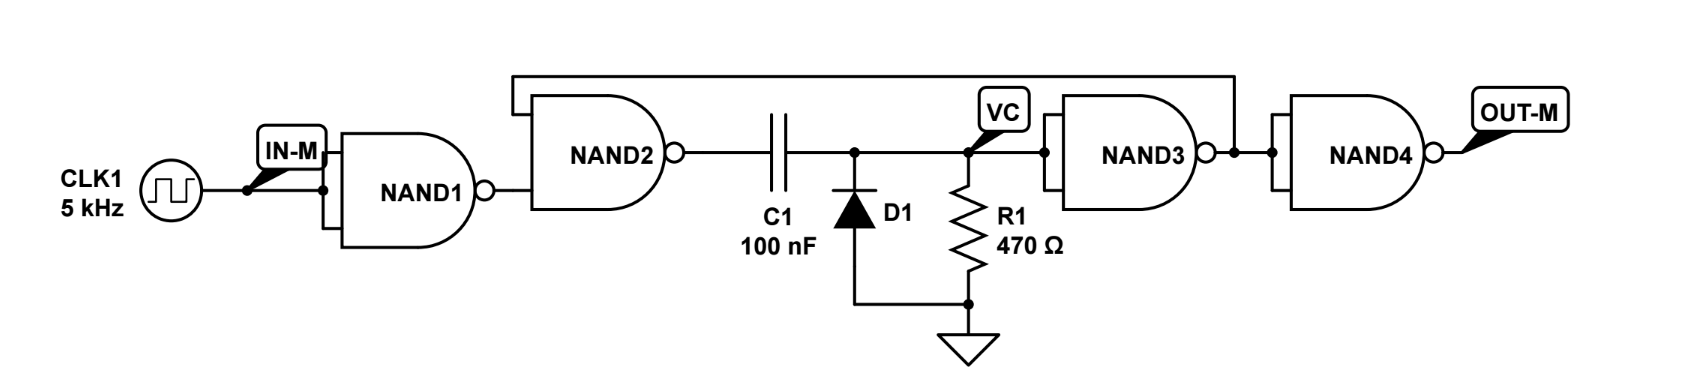
\includegraphics[scale=0.3]{monostabbo.png}
		\caption{Multivibratore monostabile.}
		\label{monocazzo}
	\end{minipage}
	\begin{minipage}{0.1\textwidth}
		\begin{tabular}{l}
			$R_1 = \SI{464(5)}{\ohm}$\\
			$C_1 = \SI{105(4)}{\nano \farad}$
		\end{tabular}
	\end{minipage}
\end{figure}

Si è verificato che il segnale in uscita fosse un onda quadra con fronte
di salita corrispondente a quello del segnale di clock in ingresso ed una durata
della semionda alta indipendente da quella del clock, come visibile in \fig{monoinout}.

\begin{figure}[H]
	\centering
	\begin{minipage}{0.3\textwidth}
		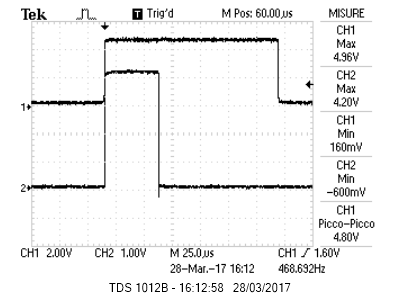
\includegraphics[scale=0.6]{monostabile_inout_500hz.png}
	\end{minipage}
	\begin{minipage}{0.3\textwidth}
		\centering
		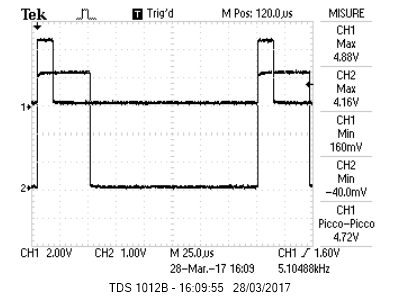
\includegraphics[scale=0.6]{monostabile_inout.png}
	\end{minipage}
	\begin{minipage}{0.3\textwidth}
		\centering
		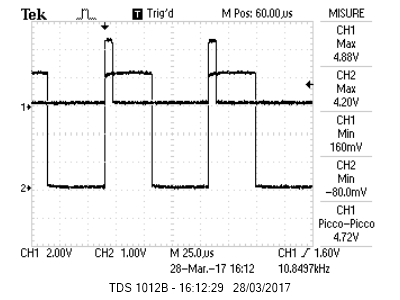
\includegraphics[scale=0.6]{monostabile_inout_10khz.png}
	\end{minipage}
	\caption{OUT-M (canale 2) e IN-M (canale 1) del multivibratore monostabile.}
	\label{monoinout}
\end{figure}

Si è dunque osservato il segnale VC in ingresso alla porta NAND3 nei due casi di
clock con semionda alta più breve e più lunga di quella del circuito
monostabile, come si riporta in \fig{monoscarica}: la tensione VC varia tra \SI{3.40(8)}{\V} e \SI{-0.64(2)}{\V}, e la commutazione del circuito avviene a  \SI{1.43(3)}{\V}.

\begin{figure}[H]
	\centering
	\begin{minipage}{0.47\textwidth}
		\centering
		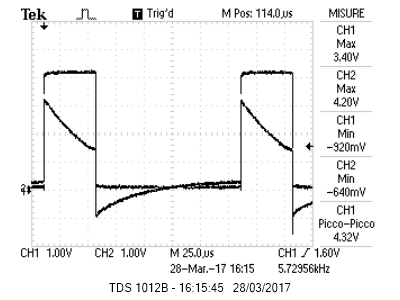
\includegraphics[scale=0.8]{monostabile_scarica.png}
	\end{minipage}
	\begin{minipage}{0.47\textwidth}
		\centering
		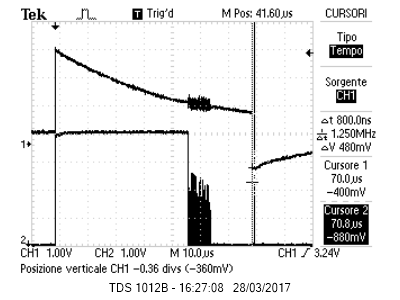
\includegraphics[scale=0.8]{monostabile_scaricaconcazzi.png}
	\end{minipage}
	\caption{OUT-M (canale 2) e VC (canale 1) del multivibratore monostabile.}
	\label{monoscarica}
\end{figure}

\subsection{Analisi del funzionamento}

In assenza di clock, il circuito mantiene output LOW: l'uscita di NAND1 è HIGH,
così come quella di NAND3, e NAND2 mantiene dunque un'uscita LOW,
ovvero prossima agli \SI{0}{\V}, e in assenza di corrente lungo $R_1$ non c'è
dunque $\Delta V$ (e di conseguenza carica) sul condensatore, cosicché anche
l'ingresso di NAND3 è LOW. Introducendo un
segnale di clock, al fronte di salita vediamo l'output di NAND1 passare a LOW e
pertanto NAND2 commuta allo stato di output HIGH: la variazione impulsiva di
tensione si trasmette attraverso il condensatore all'ingresso di NAND3, il cui
output passa dunque a LOW, portando OUT-M a HIGH. A questo punto lo stato
del clock è essenzialmente ininfluente, poiché il secondo input di NAND2 è
proprio l'output di NAND3, dunque lo stato di NAND2 non può variare fintantoché
quello di NAND3 non varia.

Poiché VC si trova ora a tensione positiva, si ha una corrente attraverso $R_1$
che porta carica sul condensatore, introducendo un $\Delta V$ ai suoi
capi e riducendo dunque la tensione a VC; quando quest'ultima scende abbastanza
da essere riconosciuta da NAND3 come un segnale LOW si ha la commutazione di
NAND3, che porta dunque allo stato LOW l'output del circuito monostabile.

In questo momento si osserva un comportamento leggermente diverso a seconda
dello stato del clock, come si osserva in \fig{monoscarica}: se il clock è già tornato LOW, la commutazione di NAND3
porta anche NAND2 a transire ad output LOW, dunque VC scende pressoché
istantaneamente ad una tensione negativa (rapidamente riportata alla tensione
di soglia del diodo dalla corrente che attraverso esso scarica velocemente il
condensatore), per poi risalire lentamente con la scarica di $C_1$ attraverso
$R_1$, e nessuna delle porte NAND cambia dunque il proprio stato.
Se al contrario il clock è ancora HIGH, e dunque l'uscita di NAND1 ancora LOW,
alla commutazione di NAND3 l'uscita di NAND2 non può passare a LOW, e il variare
di una delle due tensioni in ingresso probabilmente causa una variazione verso
l'alto della tensione in uscita, che trasmettendosi
attraverso il condensatore riporta brevemente VC sopra la soglia di
commutazione di NAND3, che dunque ritorna ad un output LOW e riporta l'uscita
di NAND2 alla tensione precedente. Questo ciclo si ripete rapidamente finché
il condensatore non si è caricato a sufficienza da mantenere VC sotto soglia
anche dopo la variazione dell'output di NAND2; quest'ultimo passerà infine a
LOW (e di conseguenza VC ad una tensione negativa) al fronte di discesa del
clock.

Il ciclo si ripete al successivo fronte di salita del clock: ci aspettiamo
dunque che il periodo del segnale del multivibratore monostabile sia pari a
quello del clock in ingresso, mentre la durata ($T_H$) dello stato HIGH
dell'output dipenda unicamente da resistenza e condensatori utilizzati.

\subsection{Linearità di $T_H$ con la resistenza}

Si è variata la resistenza $R_1$ attorno ai \SI{450}{\ohm}, misurando $T_H$, per
poi procedere ad un fit lineare $T_H = a R_1 + b$, ottenendo i seguenti risultati:

$$a = \SI{0.1095(8)}{\micro\second \per \ohm} \qquad b=\SI{-3.5(4)}{\micro \second} \qquad \chi^2/ndof = 7.0/6 \qquad corr(a,b)= -0.986$$

Dati e fit sono riportati in \fig{monofit}.

\begin{figure}[h]
	\centering
	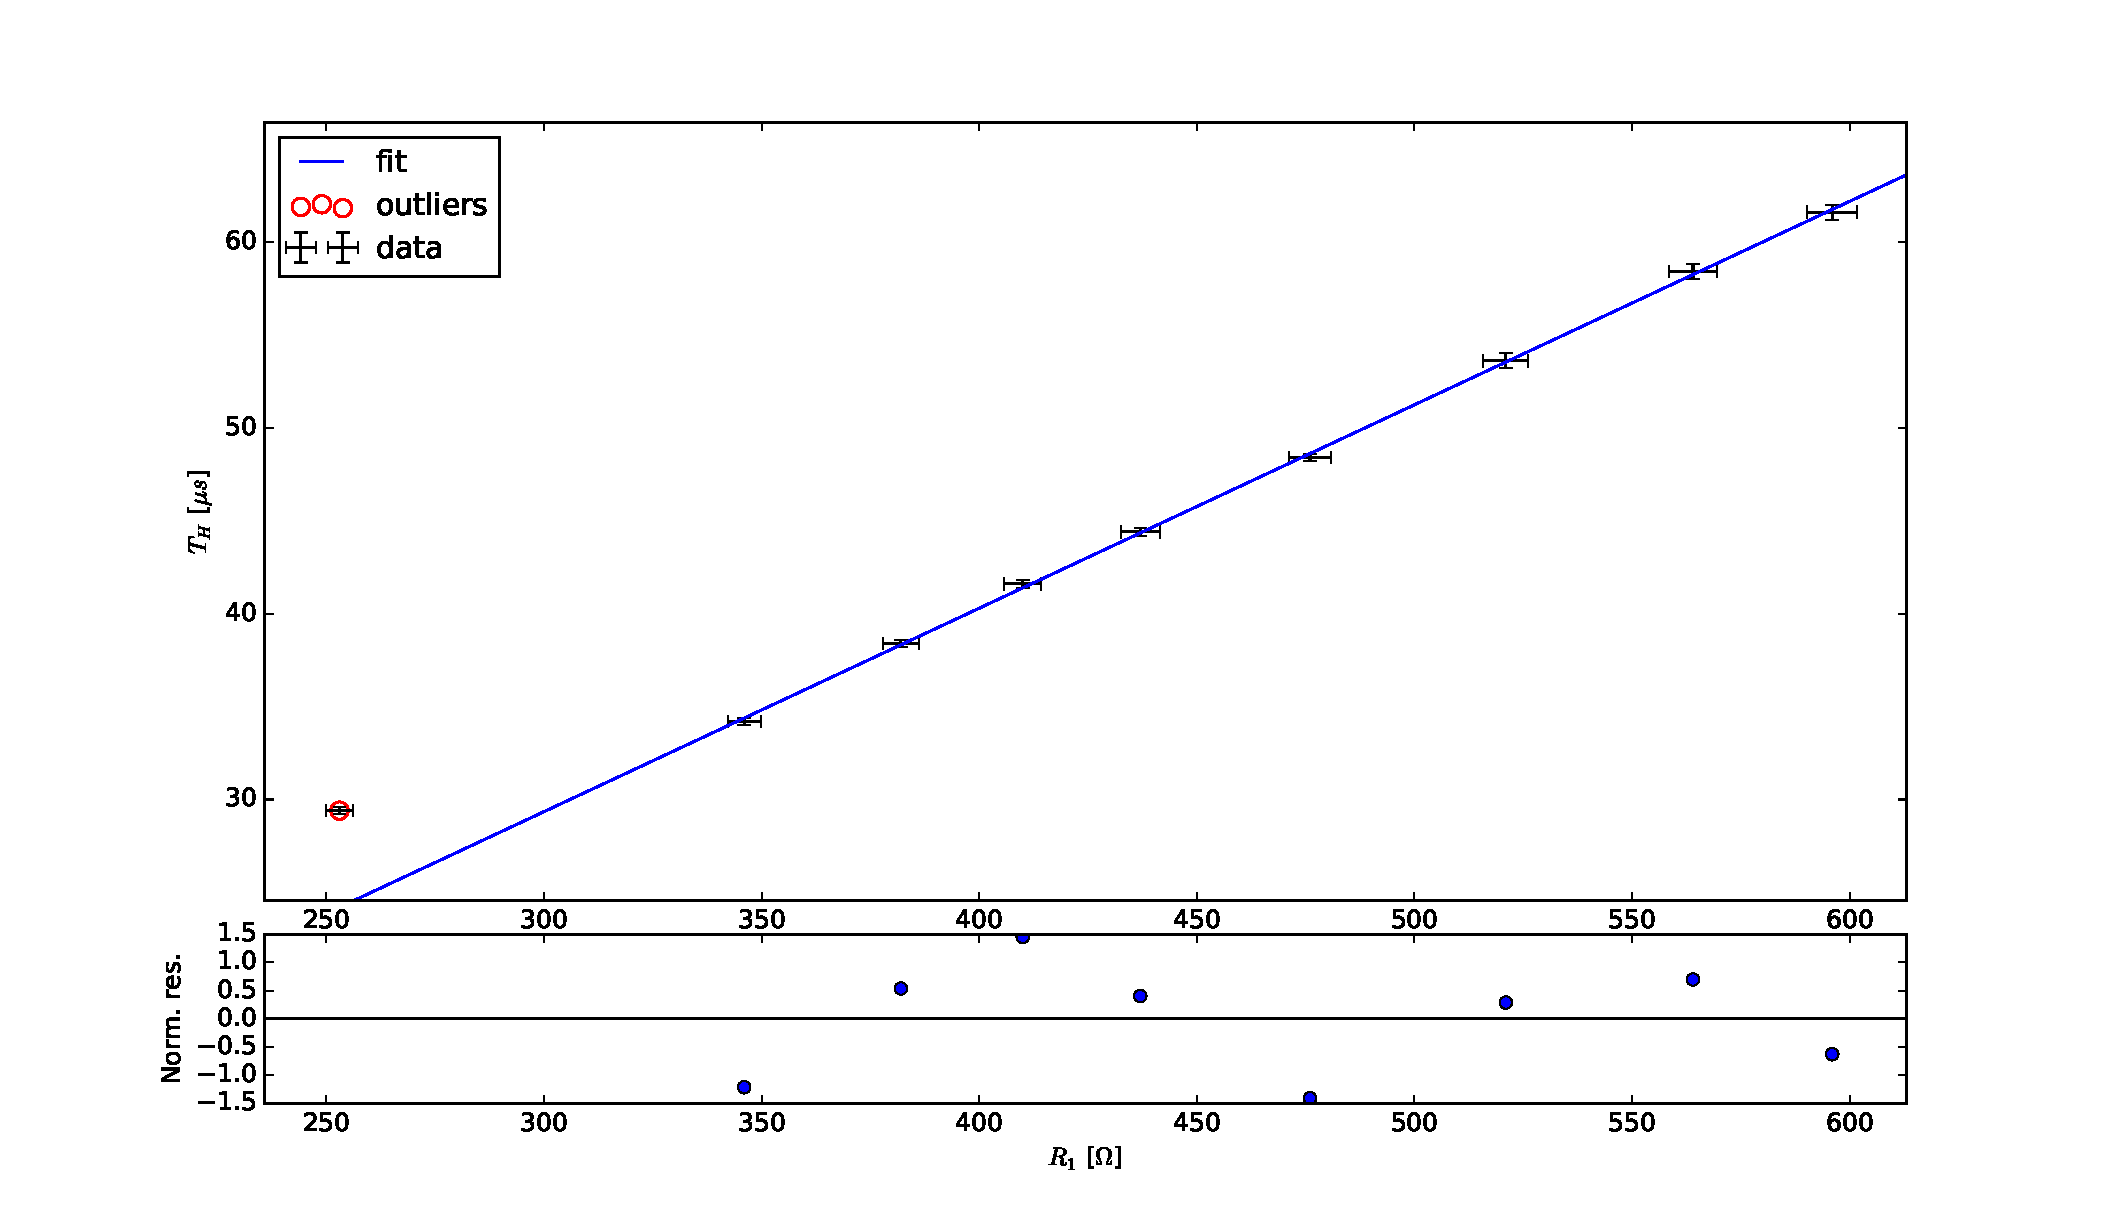
\includegraphics[scale=0.4]{monofit.pdf}
	\caption{Dati raccolti e fit della linearità del multivibratore monostabile.}
	\label{monofit}
\end{figure}
